\documentclass[12pt, a4paper]{report}
\usepackage[top=1.0in, bottom=1.0in, left=0.8in, right=0.8in]{geometry}
\usepackage{graphicx}
\usepackage{amsmath}
\usepackage{listings}
\usepackage{fancyvrb}

 	
\title{\textbf{EE2703 : Applied Programming Lab \\ Assignment 3 \\ Fitting Data to Models}} 
\author{Aditya Nanda Kishore\\ EE20B062} 

\date{\today} % Date for the report

	
\begin{document}		
\maketitle
\section{Abstract}
The aim of this assignment is to read data from a data set and drawing a best fit plot through the data set, We learn how to Extract Information from. a given data array, Plotting Graphs, and Labels, Understanding how noise addition and extraction works, Modelling the data through Least Mean Square Method and in summary we learn about some tools that play an important role in broad topics such as digression. 



\section{Introduction}
We are given a code that outputs a data set. We have to extract data from that file and read it, we have to plot and label the required attributes, We later plot Error bars with the true values and We Construct two matrices, one with Bessel function, time and another with our data with noise. Later, we use special commands to solve the matrices and find the perfect fit for our model using least mean squared error method, we later plot the graph in log scale for better understanding of what's happening there.

\section{Assignment}
\subsection{ Q1 and Q2}
% When adding * to \section, \subsection, etc... LaTeX will not assign
% a number to the section
Importing the standard libraries
\begin{Verbatim}
from pylab import *
import scipy.special as sp
import numpy as np
import matplotlib.pyplot as ax
\end{Verbatim}

The code given generates \textbf{fitting.dat}, whose first column is time, while the remaining columns are data. We separate them by

\begin{Verbatim}
f = np.loadtxt("fitting.dat", dtype = float)
time, data = f[:,0], f[:, 1:] #data_arr has just the data with time extracted
\end{Verbatim}
\subsection{Q3}
Now we plot the function for various noise amounts, as well as the true function and add labels to each function. Every column in the master matrix acts a  different function here.
\begin{Verbatim}

A0 = 1.05
B0 = -0.105

y = g(t, A0, B0)
Y=meshgrid( y, ones(k),indexing = 'ij')[0] 
scl=logspace(-1,-3,k)  # noise stdev
n=dot(randn(N,k),diag(scl))
yy=Y+n    


plot(t,yy)
xlabel( r'$t$' , size=20 )
ylabel(r'$f(t)+n$',size=20)
title(r'Q1,Q3 Plot')
grid(True)
ax.legend(scl)
ax.show() 
savetxt("fitting.dat",c_[t,yy]) 
show()


\end{Verbatim}


\begin{figure}[!tbh]
   	\centering
   	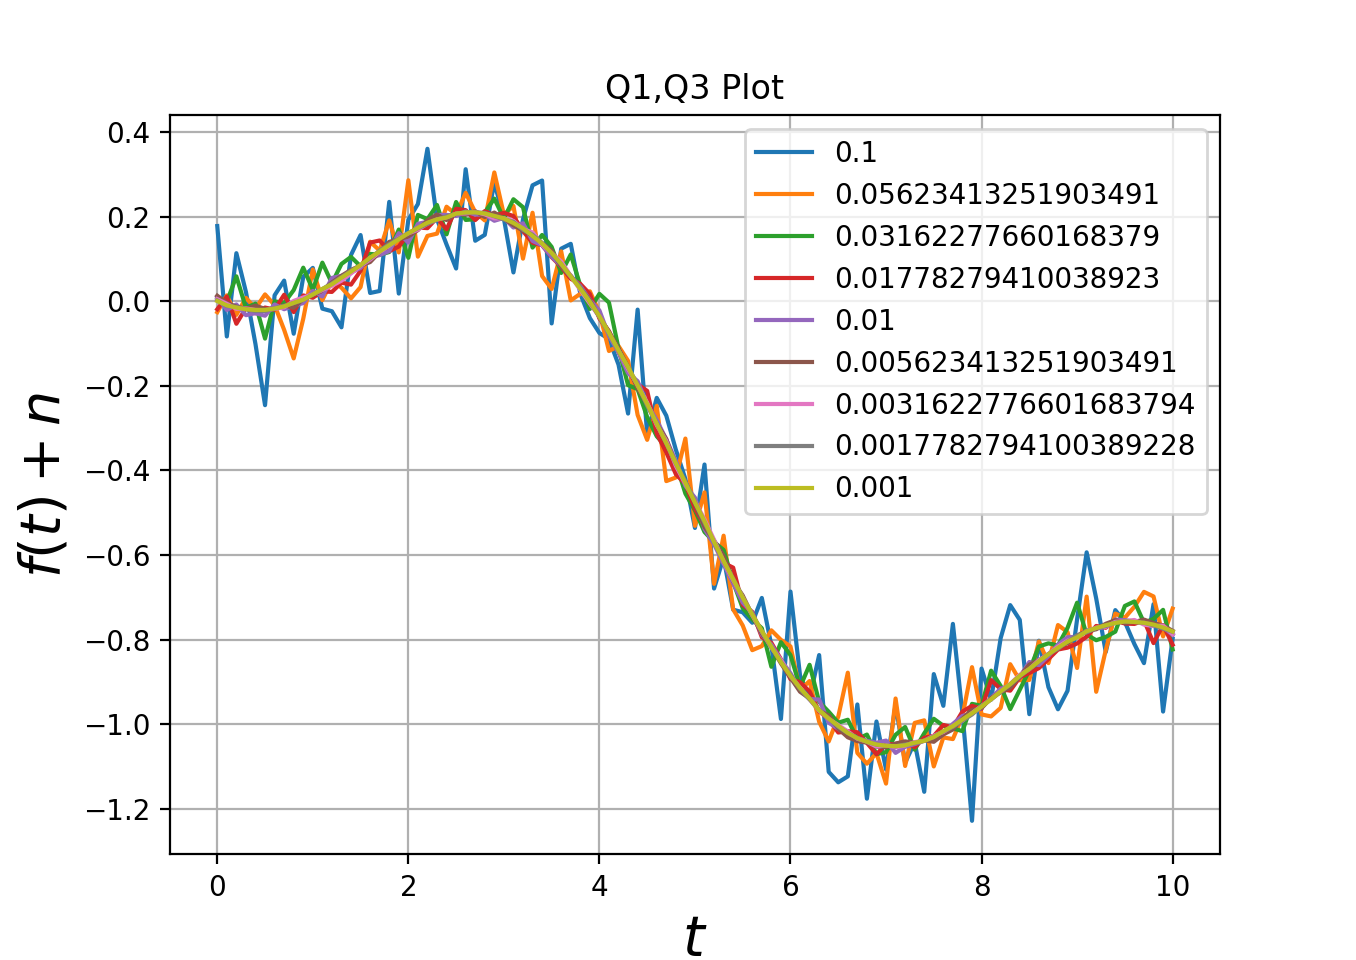
\includegraphics[scale=0.5]{Qn3.png}
   	\caption{Time vs Value, for various error amounts}
   	\label{fig:allgraphs}
   \end{figure} 

 \subsection{Q4}
 
 \begin{figure}[!tbh]
   	\centering
   	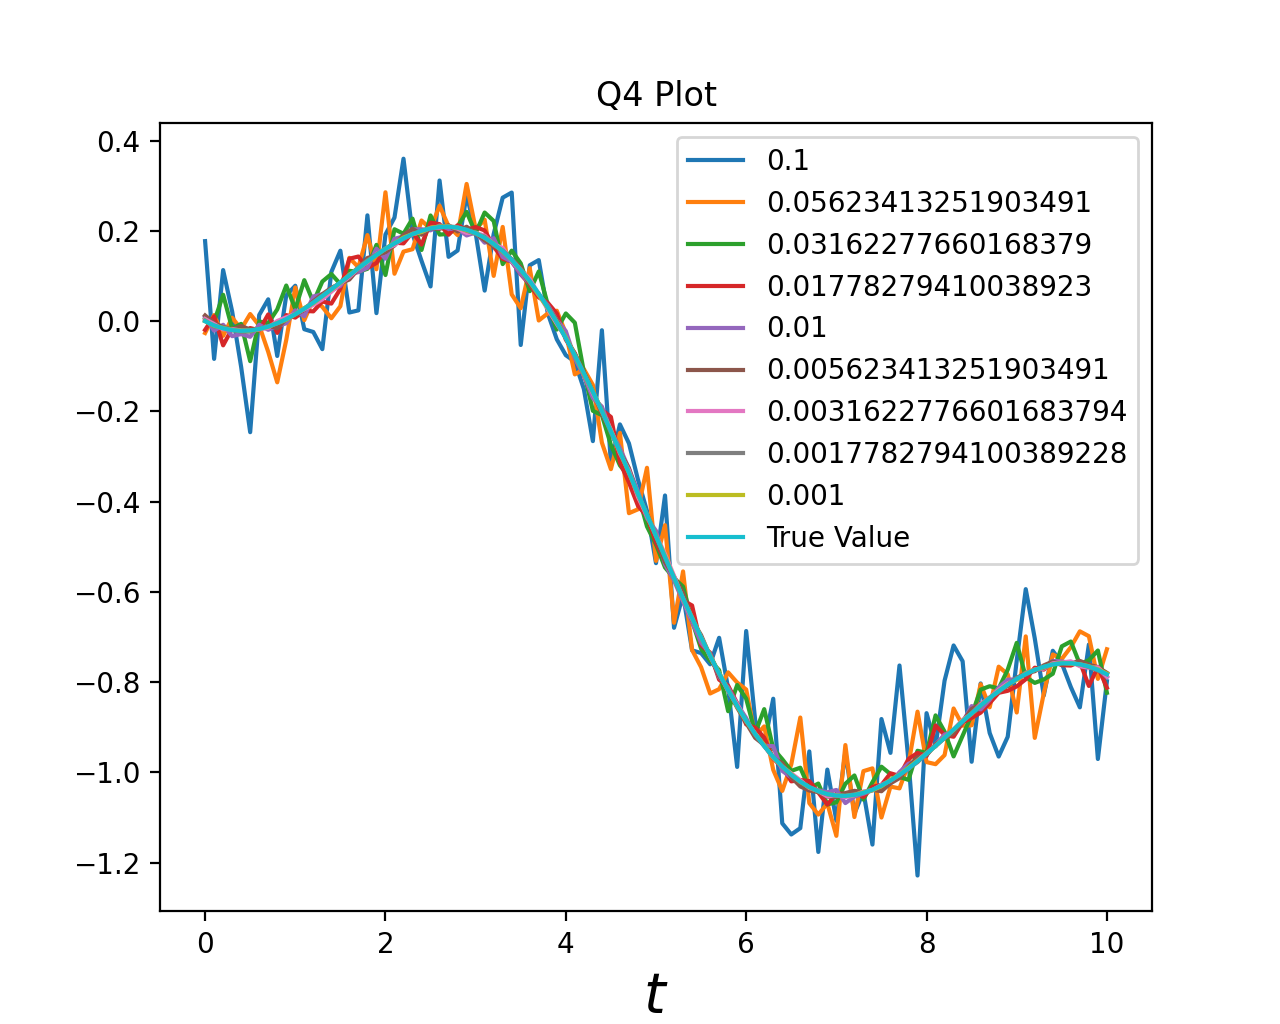
\includegraphics[scale=0.5]{Qn4.png}
	\caption{Time vs Value, for various error amounts with True Value}
   	\label{fig:trueNoMatrix}
 \end{figure}
The function is defined as follows
\begin{Verbatim}
def g(t,A,B):
    true_val =A*sp.jn(2,t)+B*t 
    return true_val
\end{Verbatim}
Now that function is defined you can plot the function with "True Value"  as a new Label
 \begin{Verbatim}
yy = np.hstack((yy, np.atleast_2d(y).T))
plot(t, yy)
xlabel( r'$t$' , size=20 )
title(r'Q4 Plot')
ax.legend(list(scl) + ["True Value"])
ax.show() 
\end{Verbatim}
   
  
 \subsection{Q5}
Now we draw a plot with Error Bars at consecutive intervals
 \begin{Verbatim}
stdev = scl[0]
errorbar(t[::5],(data.T[0])[::5],stdev,fmt='ro')
plot(t, (yy.T)[-1])
xlabel( r'$t$' , size=20 )
title(r'Q5 Plot')
ax.legend(['g(t,A,B)', 'Error Bar'])
show()
\end{Verbatim}

\begin{figure}[!tbh]
   	\centering
   	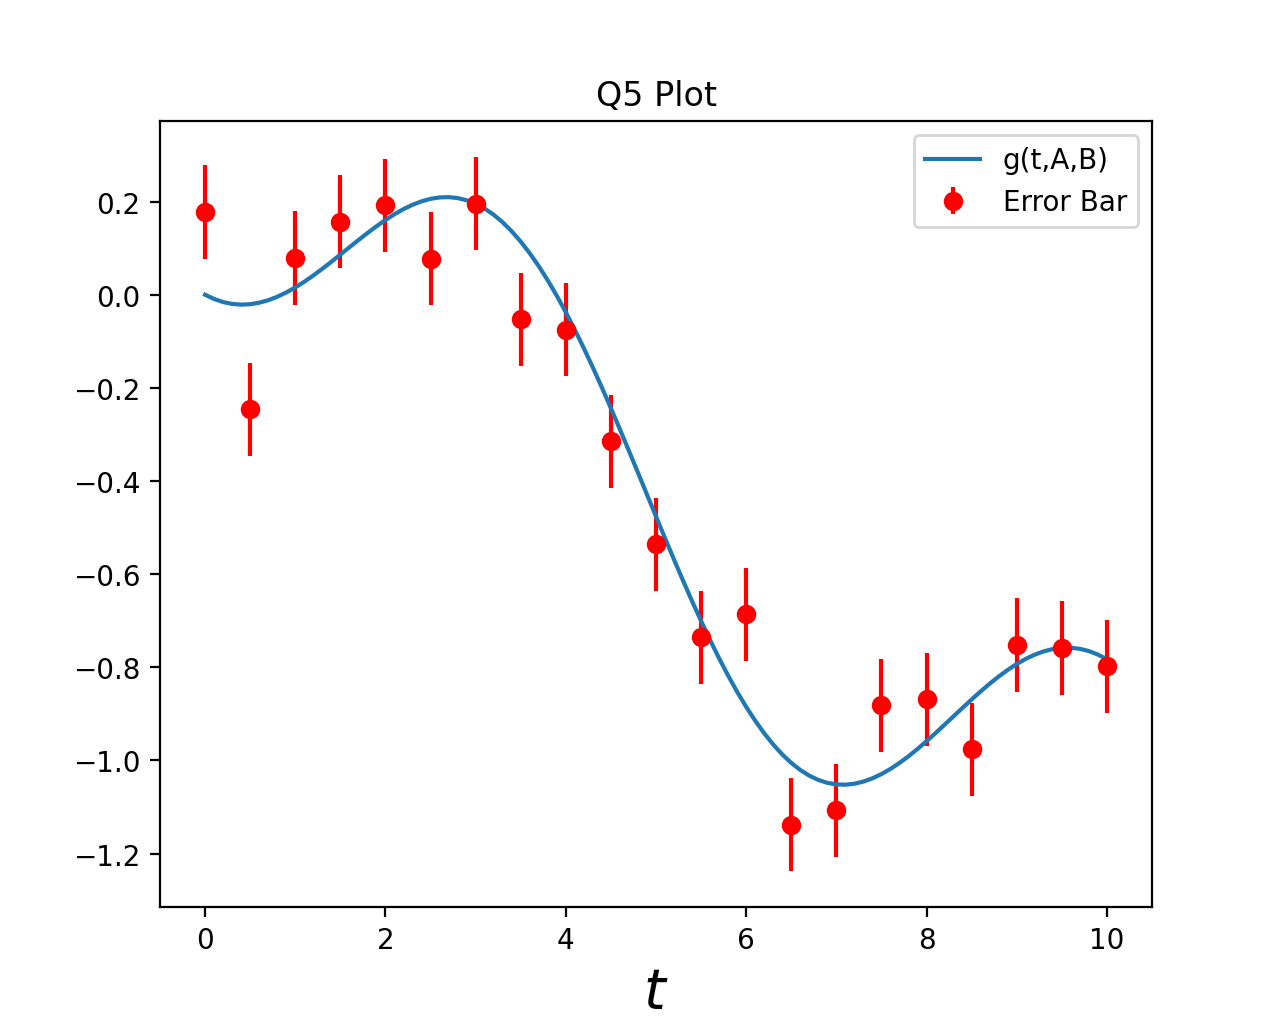
\includegraphics[scale=0.5]{Qn5.png}
   	\caption{Function with Error Bars}
   	\label{fig:errorbars}
   \end{figure}

  
 \subsection{Q6}
If we observe our estimated function carefully, It can be written as multiplication of two matrices just as given in the question, One comprising of Bessel function and time intervals and another comprising of $A_0$ and $B_0$. Now to compare both functions there are two ways, One can be subtracting two arrays and verifying if array resulted is a zero array. Another method is to plot difference of both curves and see if it's zero I would like to go with latter cause it's more fun!
 \begin{Verbatim}
 
M_1 = t
M_0 = sp.jn(2,t)
M = np.c_[M_0, M_1]
A = np.array([A0,B0])
B = np.dot(M, A.T)
B = np.c_[B.T-y, y] #checking if they are same or not
plot(t, B)
title(r'Q6- Plot to check whether they are same plots')
ax.legend(['g(t,A,B)-g(t,A0,B0) ', 'g(t,A0,B0)'])
show()


\end{Verbatim}

We can see that they are coinciding clearly, because the difference graph is at zero.

\begin{figure}[!tbh]
   	\centering
   	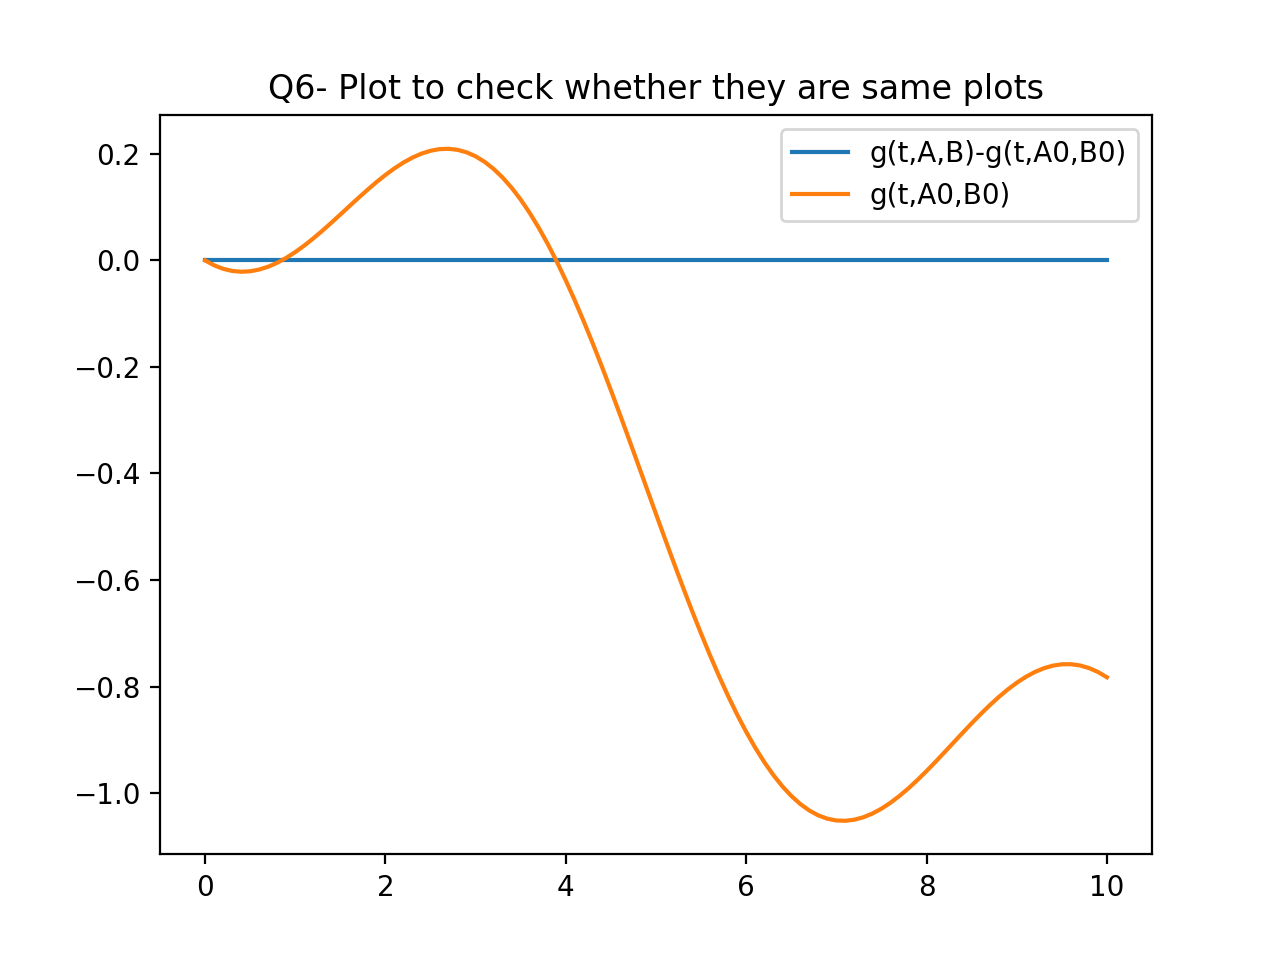
\includegraphics[scale=0.5]{Qn6.png}
	\caption{Function found using Matrix Multiplication}
   	\label{fig:trueMatrix}
   \end{figure}

 \subsection{Q7}
 We need to build the MSE matrix here for first column of our data set. So , I created two arrays for X and Y axes, A zero matrix and Using Two for loops and the given MSE function I kept amending the matrix which gave me diff values of MSEs for different A,B.
 
 \begin{Verbatim}

f = data.T[0]
A = linspace(0,2,21)
B = linspace(-0.2,0,21)
def eij_form(A,B,f):
    E = np.zeros((21,21))
    for i in range(0,21):
        for j in range(0,21):
            sum = 0
            gij = g(t,A[i],B[j])
            sum = np.dot((f - gij), (f-gij).T)
            E[i][j] = float(sum)/101
    return E
\end{Verbatim}

 \subsection{Q8}
 Plotting the contour for the Matrix created in Q7
 
 \begin{Verbatim}

ax.contour(A, B, eij_form(A,B,f))
ax.contourf(A, B, eij_form(A,B,f))
xlabel( r'$A$' , size=20 )
ylabel(r'$B$',size=20)
title(r'Q8 Contour Plot')
ax.show()
\end{Verbatim}

\begin{figure}[!tbh]
   	\centering
   	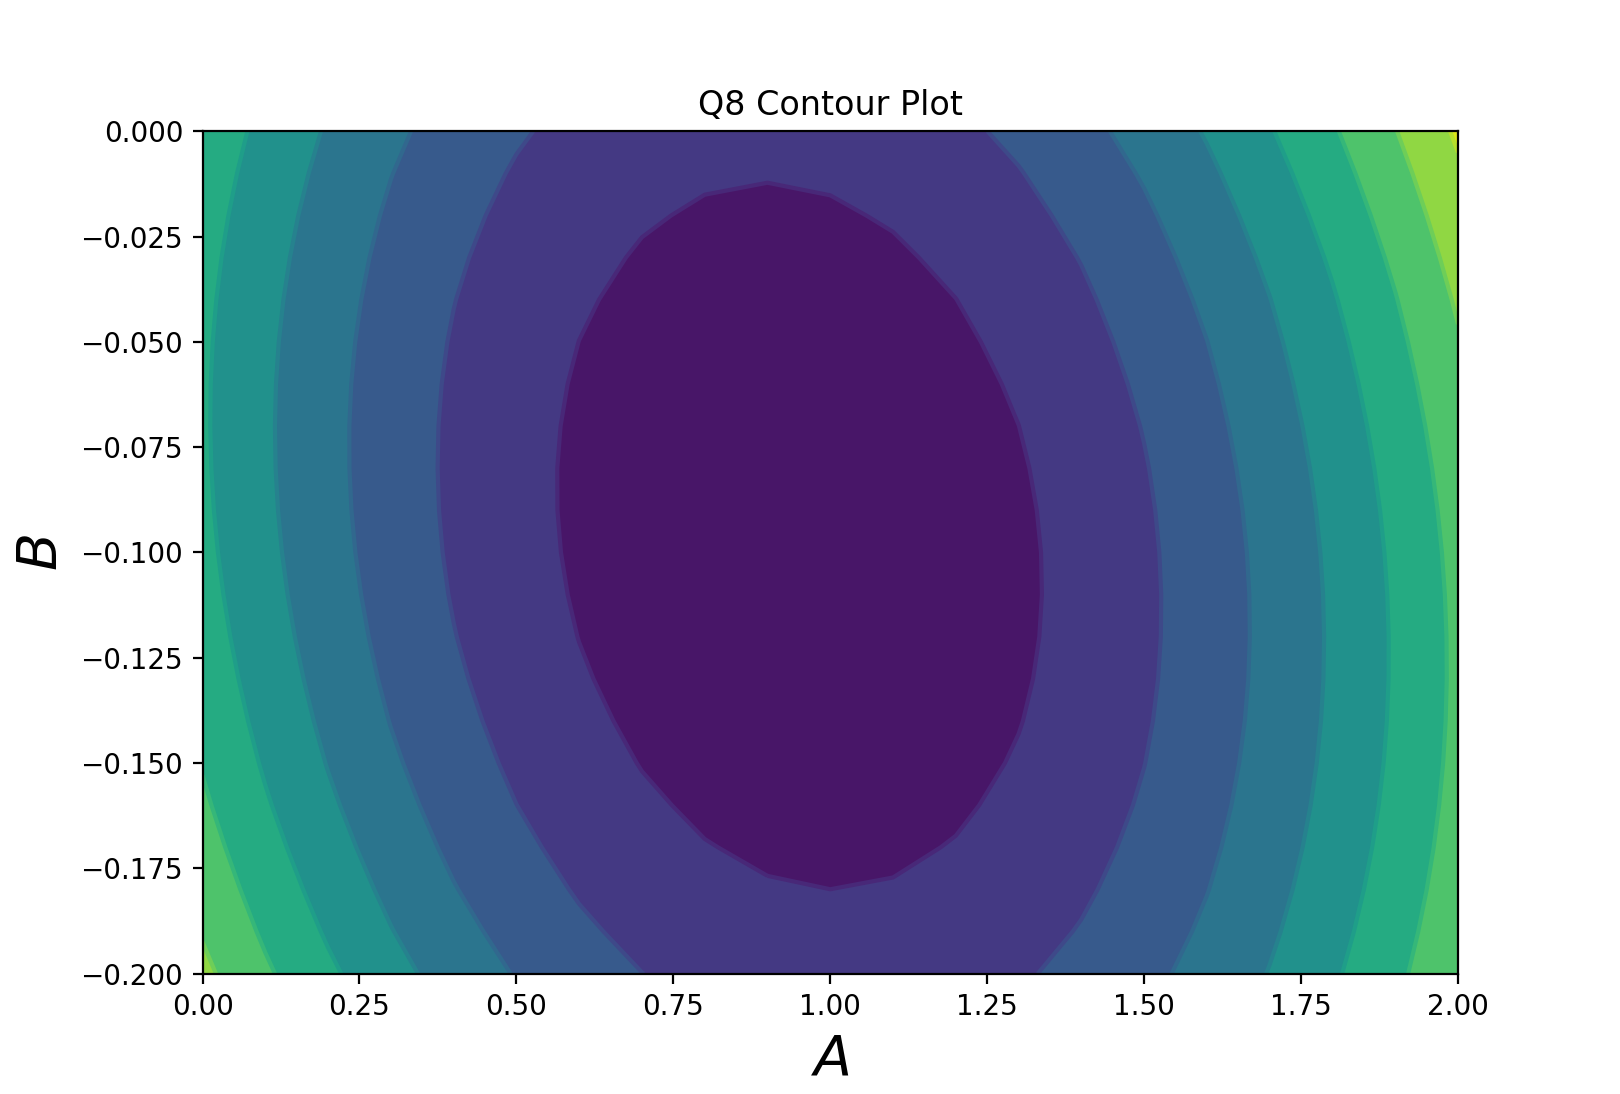
\includegraphics[scale=0.5]{Qn8.png}
   	\caption{Contour Plot of $\epsilon_{ij}$}
   	\label{fig:sample}
   \end{figure}

We can see that Contour Plot has one minima.

 \subsection{Q9}
 Here, I used the lstsq function to solve the matrix formed in Q6 and the actual function, So the expected answer here should be A = \textit{1.05} and B = \textit{-0.105}. Printing gave me that, didn't include it in the code as it's unnecessary
  \begin{Verbatim}
  
final_sol, lmse, *c = np.linalg.lstsq(M, y.T, rcond=None)

\end{Verbatim}

 \subsection{Q10}
 After repeating this for every column and finding the A,B, We can see that they are not same as $A_0$ and $B_0$. So, I made a new matrix with 2 columns, Absolute Error in A and Absolute Error in B and plotted the graph
  \begin{Verbatim}
  
error = np.zeros((k,2))
lmse = np.zeros((k,))
for i in range(0,k):
    f = data.T[i]
    E = eij_form(A,B,f)
    sol, lmse[i], *c = np.linalg.lstsq(M, f.T, rcond = None)
    error[i] = [abs(sol[0] - A0), abs(sol[1]-B0)]

plot(scl, ((error.T)[0]).T,'ro')
plot(scl, ((error.T)[1]).T,'bo')
plot(scl, lmse)
xlabel( r'$Noise$' , size=20 )
title(r'Q10 Plot')
ax.legend(['Error in A', 'Error in B', 'lmse'])
ax.show()

\end{Verbatim}
 
\begin{figure}[!tbh]
   	\centering
   	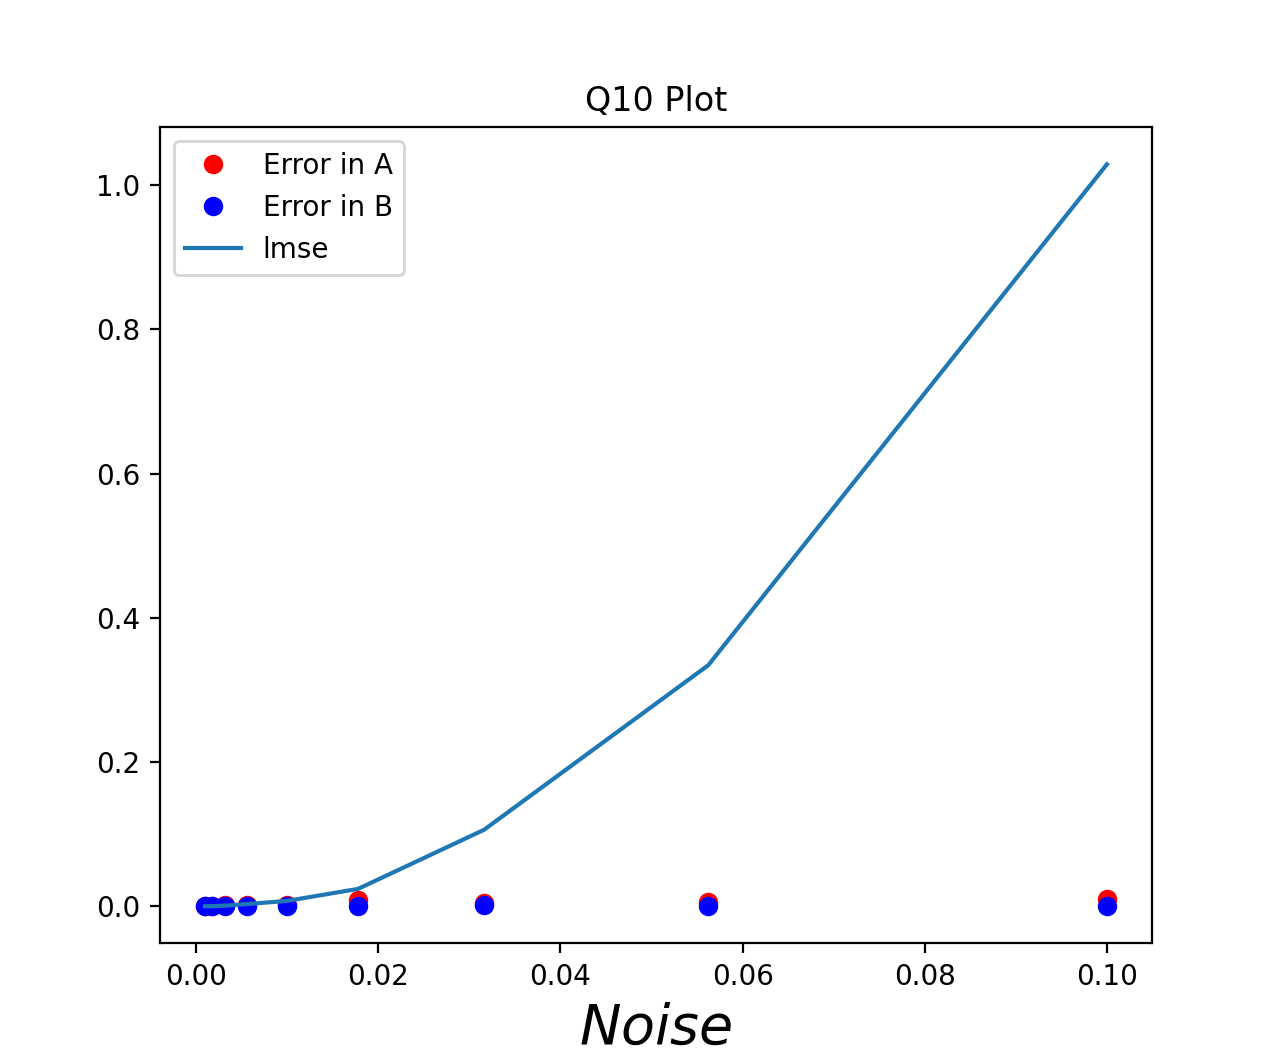
\includegraphics[scale=0.5]{Qn10.png}
   	\caption{Absolute error vs scl}
   	\label{fig:EVN}
   \end{figure}


 \subsection{Q11}
 \begin{figure}[!tbh]
   	\centering
   	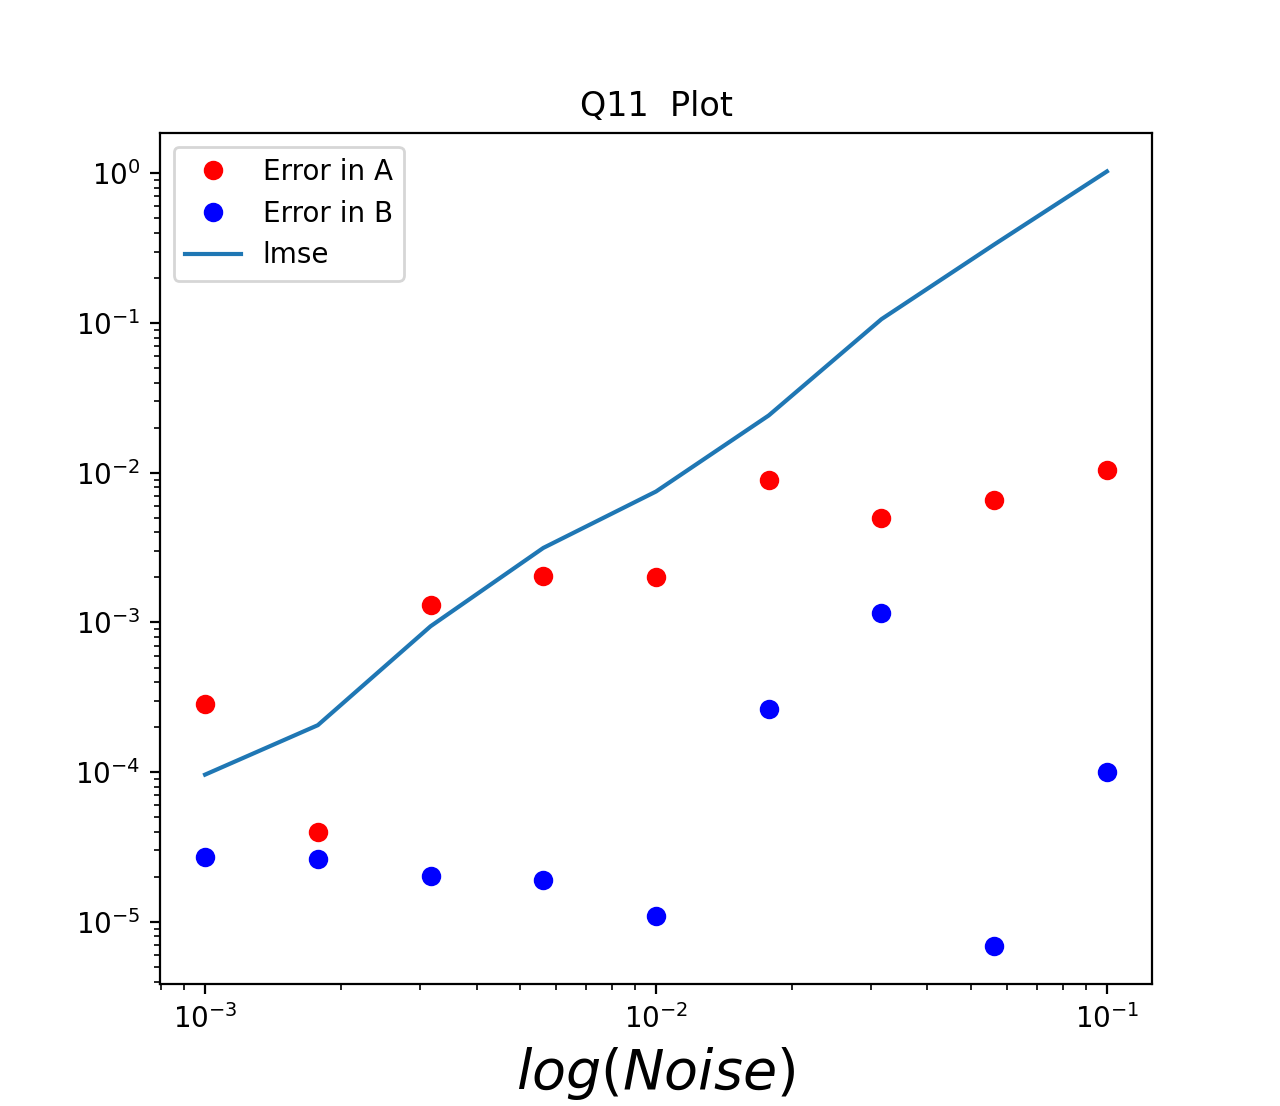
\includegraphics[scale=0.5]{Qn11.png}
   	\caption{Log(Absolute Error)vs Log(Noise)}
   	\label{fig:loglog}
   \end{figure}
I just drew the same graph in log-log plot now
 \begin{Verbatim}
loglog(scl, ((error.T)[0]).T,'ro')
loglog(scl, ((error.T)[1]).T,'bo')
loglog(scl, lmse)
xlabel( r'$log(Noise)$' , size=20 )
title(r'Q11  Plot')
ax.legend(['Error in A', 'Error in B', 'lmse'])
ax.show()
\end{Verbatim}
Clearly, We can see that log(scl) is linear with respect to noise, which is shown by the blue line.

\section{Conclusions}
\begin{itemize}
   \item The Minima of the contour plot gives us the A,B for which mean squared is the minimum indirectly giving us the "close to optimum" A,B for our function.
    \item In Plot of Q10, We can see that B varies very little when compared to A.
    \item There is only one minima in contour plot, We can get multiple minimas for more complex function estimations, but for this estimation we will only have one minima
    \item $\log(error in estimate)$ is linear with respect to $\log(noise)$.
    \item Least square method can be used for fitting a data set.
\end{itemize}
I have learnt how to plot different kinds of graphs, adding them labels, estimating the function model, calculating error and finding how error is varying with noise, so that we can have a more clear idea of how our actual function is.
\end{document}

